\chapter{Einleitung}

Heutzutage spielen Daten und deren Verarbeitung in vielen Bereichen eine immer wichtigere Rolle.
Im \textit{Rethink Data Report 2020} \textcite{rethink_data_2020} wurde eine Studie durchgeführt, die eine Steigerung von 42\% der Menge an anfallenden Daten pro Jahr prognostiziert.
Dies wird unter anderem auf den vermehrten Einsatz von IoT-Geräten, immer ausführlichere Datenanalysen und die einfachere werdende Anwendung von Cloud-Speichern zurückgeführt.
Dabei besteht die Herausforderung, Daten in verschiedensten Formaten in großen Mengen zu verwalten und zu verwenden.

Als eine Lösung für das Problem haben sich Data-Lake-Systeme hervorgetan.
Ein Data Lake ist eine Methodik, die die Erfassung, Verfeinerung, Archivierung und Erkundung von Daten verbessert \parencite{datalake_01}.
Große Datenmengen sollen möglichst kostensparend gespeichert werden.
Verschiedenste Formate können in einem Data Lake abgelegt und verarbeitet werden.
Darunter zählen zum Beispiel strukturierte Daten aus traditionellen Datenbanksystemen, semistrukturierte Daten wie JSON-Dateien, bei denen nicht alle Attribute festgelegt sind und unstrukturierte Daten wie Bilder oder Videos \parencite{datalake_02}.


\section{Zielsetzung der Arbeit}

In einer Reihe von Projekten und Masterarbeiten wird an der Hochschule Niederrhein ein generelles Data-Lake-System entwickelt.
Das heißt es ist überall einsetzbar und alle nötigen Komponenten sind im System enthalten.
Ein Prototyp wurde bereits während eines Masterprojekts entwickelt \parencite{prototyp}.

Diese Masterarbeit befasst sich mit der Entwicklung, Implementierung und Integration einer neuen Schnittstelle für die Aufnahme von Daten (Ingestion).
Die wichtigsten Ziele sind dabei die Generalität, Kontinuität und Datenversionierung bei einer möglichst einfachen Verwendung für den Benutzer.
Die Generalität bezeichnet die Funktionalität unabhängig von der Art der Datenquelle oder der Struktur der Daten.
Unter Kontinuität ist das erneute und optional auch regelmäßige Nachladen von Daten aus einer Quelle gemeint.
Für diese Daten soll es auch möglich sein eine Versionierung durch zu führen um Änderungen auswerten zu können.

Der Aufbau der Arbeit gliedert sich in fünf Kapitel.
In diesem Kapitel werden wichtige Grundlagen für die Arbeit vermittelt und verwandte Arbeiten erläutert.
Danach wird auf die Ziele und die daraus folgenden Anforderungen an die Schnittstelle eingegangen.
Das nächste Kapitel befasst sich mit der Entwicklung einer Architektur und des Designs der Ingestion.
Auf diesem Design baut die darauf folgende Umsetzung auf.
Zuletzt wird das System durch funktionale Tests und Benchmarks evaluiert.

\section{Grundlagen und Verwandte Arbeiten}

% Techniken
\subsection{Apache Spark}
\label{sec:spark}

Apache Spark ist eine Datenverabeitungs-Engine.
Das ist Ziel ist die Vereinheitlichung von Arbeitsabläufen.
Darunter fallen zum Beispiel Arbeiten mit SQL, Datenströmen, maschinellem Lernen oder Graphen-Daten.
Es gibt Bibliotheken für diese oder andere Arbeitsabläufe, die durch ihre Optimierung in Spark ähnliche Performance, wie spezialisierte Engines erreichen.
Spark kann entweder lokal auf einem Computer oder auf einem Spark-Cluster nach dem Master-Worker-Modell ausgeführt werden.

Ein Kernprinzip ist die Abstraktion der Daten in RDDs (Resilient Distributed Datasets, deutsch: Robuste Verteilte Datensätze).
RDDs sind fehlertolerante Sammlungen von Objekten, die auf den Workern verteilt werden und parallel bearbeitet werden können.
Diese werden flüchtig im Speicher gehalten, können aber für einen schnelleren Zugriff zwischengespeichert werden.
Die Erstellung und Bearbeitung von RDDs geschieht über sogenannte Transformationen.
Die Transformationen werden in einem Herkunftsgraphen gespeichert, wodurch eine Wiederherstellung bei Fehler an jedem Punkt möglich ist.

Für die Verarbeitung von strukturierten oder semi-strukturierten Daten gibt es zusätzlich die eigene Abfragesprache SparkSQL.
Spark biete APIs für die Sprachen Scala, Java, Python und R.
Auf den RDDs gibt es noch eine weitere Abstraktionsebene.
Mit DataFrames, die eine Sammlung RDDs von Datensätzen mit einem bekannten Schema sind, kann eine API benutzt werden, bei der die Bearbeitung der Daten über Funktionsaufrufe statt SparkSQL möglich ist \parencite{spark}.

Die Interaktion mit einem Spark Cluster kann über eine interaktive Shell oder als fertige Anwendung geschehen.
Informationen über die Anwendung werden im SparkContext gespeichert.
Beim Lesen und Schreiben wird das Format der Daten angegeben.
Spark unterstützt standardmäßig einige Formate, aber durch die Konfiguration von extra Bibilotheken im SparkContext, können beliebige Formate hinuzgefügt werden.
Von der verwendet Bibilothek sind auch die Optionen abhängig, die beim Lesen und Schreiben gesetzt werden müssen.
Die Optionen sind immer Schlüssel-Wert-Paare und enthalten zum Beispiel Verbindungsinformationen zu einer Datenbank oder einen Dateispeicherort \parencite{spark-website}.

\subsection{Hadoop Distributed File System}

Das Hadoop Distributed File System (HDFS) ist ein verteiltes und fehlertolerantes Dateisystem.
Es wurde entwickelt um auf Hardware mit geringen Kosten zu laufen und große Datenmengen zu verarbeiten.
Im HDFS gespeicherte Dateien können von einem Gigabyte bis mehrere Terabyte groß sein.
Die Fehlertoleranz wird dabei durch die Möglichkeit der Replikation mit einem beliebigen Faktor gegeben.

Das Dateisystem ist ähnlich zu anderen bekannten Dateisystemen.
Dateien und Ordner können im Namensraum hierarchisch organisiert werden.
Es unterstützt jedoch keine Zurgiffsberechtigung oder Hard- und Soft-Links.
Um einfach und effektiv kohärent zu bleiben, werden Dateien nur einmal geschrieben, können aber mehrfach gelesen werden.
Dateien werden zur Speicherung in einzelne Blöcke aufgeteilt.
Dabei sind für eine Datei alle, bis auf der letzte, Blöcke gleich groß.

Ein HDFS-Cluster funktioniert nach dem Master-Worker-Prinzip und besteht aus einem NameNode und vielen DataNodes.
Der NameNode übernimmt die Verwaltung des Namensraum und Verteilung der einzelnen Blöcke einer Datei.
Er reguliert dazu noch den Zugriff durch Clients und führt Operationen auf dem Dateisystem, wie das Öffnen, Schließen oder Umbenennen von Ordnern und Dateien aus.
Die DataNodes speichern die einzelnen Blöcke der Dateien.
Auf die Anweisung des NameNodes werden Blöcke erstellt, gelöscht oder repliziert.
Außerdem bearbeiten sie Anfragen zum Lesen und Schreiben von Dateien \parencite{hdfs}.

% Parquet
Mit Apache Parquet steht ein Format zur Verfügung, mit dem Daten im HDFS effizient gespeichert werden können.
Parquet ist ein spalten-orientiertes Speicherformat, das auch die Kompression und Kodierung der Daten unterstützt.
Auch die Speicherung von verschachtelten Daten ist möglich.

\subsection{Apache Kafka}

Apache Kafka ist ein verteiltes Event-Streaming-System.
Die Vermittlung von Nachrichten nach dem Publish-Subscribe-Muster läuft dabei in Echtzeit.
Events können von Produzenten veröffentlicht werden und Konsumenten können auf diese Events abonnieren.
Durch seine Verteilung kann Kafka den Ausfall einzelner Server ausgleichen.
Zusätzlich können Ströme von Events für einen beliebigen Zeitraum persistiert werden.

Kafka besteht aus einem Cluster von Servern und verschiedenen Clients.
Es gibt zwei Arten von Servern.
Die sogenannten Broaker sind für die Verteilung und Verwaltung von Events zuständig.
Andere verwenden Kafka Connect\footnote{https://kafka.apache.org/documentation/\#connect} um existierende Systeme, zum Beispiel eine Datenbank, in das Kafka Cluster zu integrieren.
Die Clients sind Anwendungen die entweder Events produzieren oder konsumieren.

In diesem System repräsentiert ein Event den Fakt, dass etwas "`passiert"' ist und besteht aus einem Schlüssel, einem Wert, einem Zeitstempel und optionalen Metadaten.
Dabei werden die Werte nicht interpretiert sonder einfach als Block versendet und können so beliebige Struktur haben.
Events werden in sogenannte Topics unterteilt.
Es kann immer mehrere Produzenten oder Konsumenten auf einer Topic geben.
Events in einer Topic können mehrfach gelesen werden und werden nicht nach dem Konsumieren gelöscht.
Es kann aber für jede Topic einzeln eine Dauer festgelegt werden, nach der die Events verworfen werden.
Um eine Topic fehlertolerant zu machen, kann diese repliziert werden.

Topics werden in Partitionen über verschiedene Broaker aufgeteilt, so dass das ganze System gut skalierbar wird.
Ein Produzenten kann zum Beispiel Events auf mehreren Brokern gleichzeitig veröffentlichen.
Wenn ein Event in einer Topic veröffentlicht wird, wird dieses an eine der Partitionen angehängt.
Events, die den gleichen Schlüssel haben werden immer der gleichen Partition zugeordnet und Events einer Partition kommen garantiert in der Reihenfolge des Schreibens bei dem Konsumenten der Partition an \parencite{kafka-docs}.
\subsection{Delta Lake}

Delta Lake ist eine extra Speicher-Ebene, die auf dem HDFS angewendet werden kann.
Das Ziel ist es diesen Speichern ACID Transaktionen, schnelles Arbeiten mit Metadaten der Tabelle und eine Versionierung der Daten hinzuzufügen.
Daten werden in sogenannten Delta Tabellen mit Metadaten und Logs gespeichert.

Eine Delta Tabelle ist ein Verzeichnis im Speicher.
Die tatsächlichen Daten werden hier in Apache Parquet Dateien abgelegt.
Parquet ist ein spalten-orientiertes Format, zum effizienten Speichern von Daten \parencite{parquet}.
Dabei können die Daten auch noch in Unterverzeichnisse aufgeteilt sein, zum Beispiel für jedes Datum ein Verzeichnis.
Neben den Datenverzeichnissen gibt es eines für die Logs in Form von JSON Dateien mit aufsteigender Nummerierung.
Metadaten werden sowohl innerhalb der Parquet als auch der Log Dateien passend gespeichert.

Im Delta Lake wird ein Protokoll für den Zugriff verwendet, dass es ermöglicht, dass mehrere Clients gleichzeitig Lesen und immer nur einer Schreiben kann.
Dabei werden beim Schreiben immer erst neue Datensätze, die zur Tabelle hinzugefügt werden sollen in das korrekte Verzeichnis geschrieben.
Danach wird eine neu Log Datei erstellt.

Beim Lesen werden die Log Dateien als Grundlage verwendet um daraus zusammen mit den gespeicherten Daten den Tabellen stand zu erzeugen.
Man kann beim Lesen auch eine bestimmte Version angeben.
Um den Aufwand bei der Verarbeitung der Logs zu verringern wird periodisch ein Kontrollpunkt erzeugt, bei dem alle vorherigen Logs zusammengefügt und komprimiert werden.
Das bedeutet, dass zum Beispiel das Operationen die sich gegenseitig aufheben nicht gespeichert werden.
Damit reicht es aus nur den letzten Checkpoint vor der zu lesenden Version und alle darauf folgende Logs zu lesen.

Durch das Design werden keine eignen Server für die Pflege der Delta Tabellen benötigt, sondern dies kann alles über den Client gemacht werden.
Der Delta Lake unterstützt sowohl die Batch-Verarbeitung von Daten als auch Datenströme und bietet volle Integration in Spark \parencite{deltalake}.



% Arbeiten
\subsection{Der Data-Lake-Prototyp}
Ein Data Lake basiert darauf, dass zuerst alle Daten in ihrem Rohformat gespeichert werden.
Dadruch fällt der Aufwand einer Transformation bei der Integration von neuen Daten weg.
Gleichzeitig bleiben auch alle Informationen bleiben für Analysen erhalten\parencite{datalake_03}.
Neben dem Speichern und Bereitstellen von Daten ist eine weitere Aufgabe eines Data-Lake-Systems die verwaltung von Metadaten.


Wärend dem Masterprojekt \citetitle{prototyp} \parencite{prototyp} an der Hochschule Niederrhein wurde bereits eine Data-Lake-System-Prototyp entwickelt.
In \fref{fig:prototyp-architektur} ist ein Überblick über dessen Architektur zu sehen.
Es handelt sich hierbei um eine Client-Server-Anwendung.
Der Client besteht aus einer Web-Anwendung über die Benutzer mit dem Data-Lake-System interagieren.
Er kommuniziert mit dem Server über eine REST-API, die auch durch andere Clients verwendet werden könnte.
Die Datenverarbeitung wird über ein Apache Spark Cluster gelöst.
Zum Speichern der Daten stehen drei verschieden System zu verfügung.
Eine Postgres Datenbank für strukturierte, eine MongoDB für semistrukturierte und ein HDFS für unstrukturierte Daten.

\begin{figure}
    \centering
    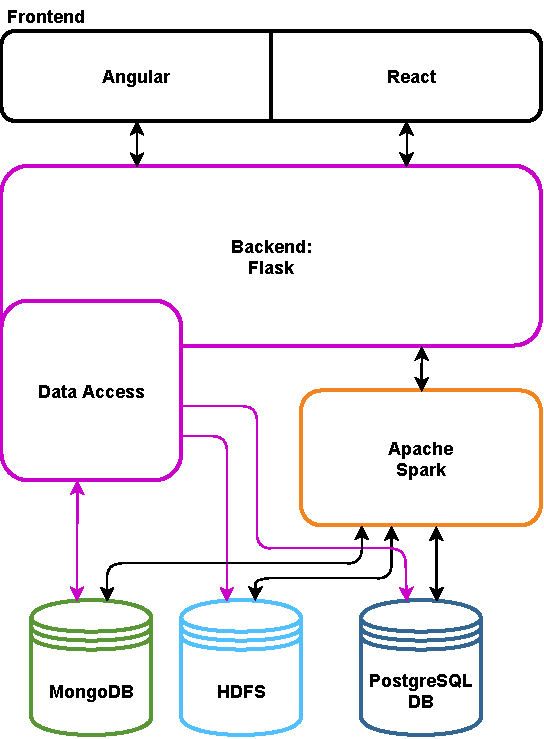
\includegraphics{Grafiken/data_lake_prototype_arch.pdf}
    \caption{Architektur des Prototypen, \citetitle[Quelle:][S. 2]{prototyp}}
    \label{fig:prototyp-architektur}
\end{figure}

Die Verarbeitung der Ingestion ist im Prototyp Abhängig von der Datenquelle und dem ausgewählten Zielspeicher.
In \fref{fig:prototyp-ingestion} sind die verschiedenen Wege zu sehen.
Diese Verarbeitungsweise hat zwei Probleme, die in der neuen Ingestion gelöst werden müssen.
Dadurch, dass der Benutzer aus den verschiedenen Speichern ein Ziel auswählt, können hier leicht Probleme entstehen, falls die Datenquelle nicht mit dem Format des Speichers kompatibel ist.
Außerdem sind die Verarbeitungsweisen der Quellen zu den Speichern fest im Code des Servers festgehalten.
So ist es nicht möglich wärend der Laufzeit neue Datenquellen zu integrieren.

\begin{figure}
    \centering
    \subfigure[Datenbank-Ingestion]{
        \label{fig:prototyp-db-ingeston}
        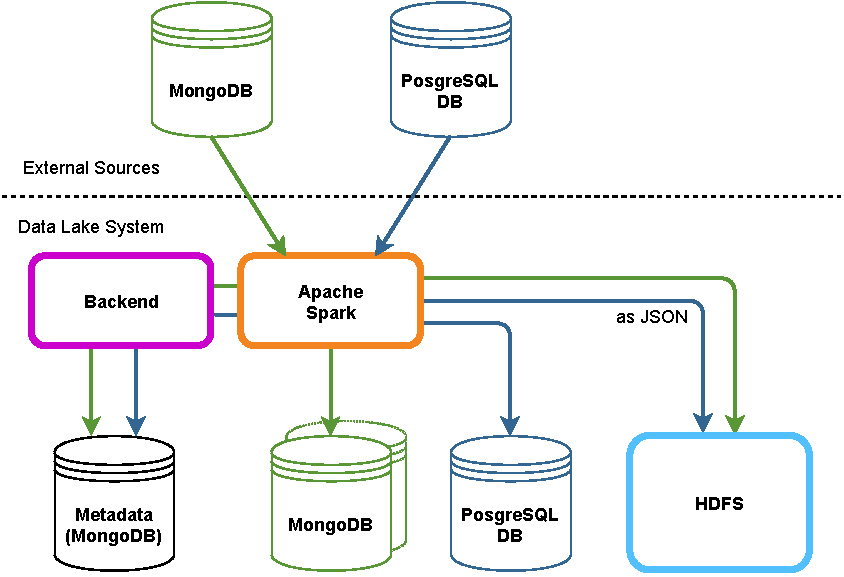
\includegraphics[width=.45\textwidth]{Grafiken/db_ingestion.pdf}
    }
    \subfigure[Datei-Ingestion]{
        \label{fig:prototyp-file-ingeston}
        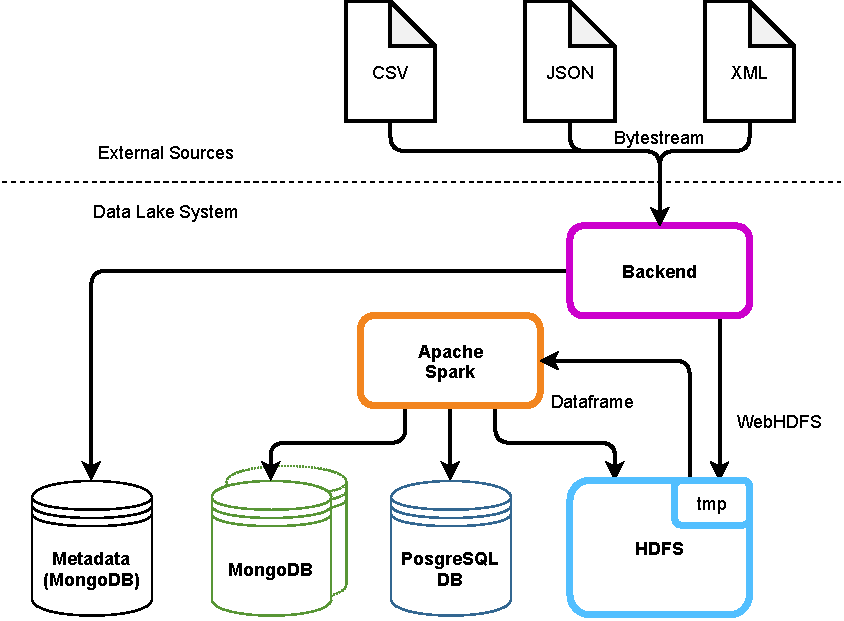
\includegraphics[width=.45\textwidth]{Grafiken/file_ingestion.pdf}
    }
    \caption{Ingestion-Verarbeitung des Prototypen, \citetitle[Quelle:][S. 3]{prototyp}}
    \label{fig:prototyp-ingestion}
\end{figure}
\subsection{Change Data Capture (CDC)}
\label{sec:cdc}

Um Änderungen an Daten in Datenquellen in das Data-Lake-System einpflegen zu können, müssen diese erst erfasst werden.
Diesen Prozess nennt man Change Data Capture (CDC).
Das Ziel beim CDC ist es, die Änderungen an den Daten nur an einer Stelle zu erfassen und dann an andere Systeme weiter zu schicken.
Dafür gibt es verschiedene Ansätze, die in den Arbeiten \citetitle{delta-view_gen}\parencite{delta-view_gen}, \citetitle{cdc_in_nosql}\parencite{cdc_in_nosql} und \citetitle{boeing}\parencite{boeing} erläutert werden.

\subsubsection{Datenbank-Trigger basiert}
Datenbank-Trigger sind Events, die bei verschiedenen Aktionen auf den Daten in einer Datenbank ausgelöst werden.
Über diese Trigger lassen sich CDC-Programme realisieren, die Änderungen genau dann festhalten, wenn sie geschehen.
Ein Nachteil ist, dass die Methode nur in System angewendet werden kann, die auch Trigger unterstützen.
Dafür ist es möglich alle Änderungen wie Einfügen, Aktualisieren oder Löschen von Daten zu erfassen \parencite{boeing}.

\subsubsection{Log basiert}
Es gibt viele Datenspeicher-Systeme, die Logs über die Aktionen auf den Daten führen.
Diese werden zum Beispiel genutzt um eine Wiederherstellung möglich zu machen.
Ein CDC-Programm kann diese Logs auslesen und daraus die Änderungsdaten erzeugen.
Hierdurch gibt es fast keinen extra Aufwand für das eigentliche System.
Aber auch hier gilt, dass diese Methode davon abhängig ist ob ein System Logs erstellt und ob diese durch externe Programme abgerufen werden können \parencite{delta-view_gen}.


\subsubsection{Zeitstempel basiert}
Ein weiterer Ansatz ist die Verwendung von Zeitstempeln mit den Zeitpunkten der Erstellung und letzten Änderung.
Diese Zeitstempel müssen jedem Datensatz vorhanden sein.
Die Verantwortung dafür kann entweder bei dem Ersteller der Daten liegen oder durch das Speichersystem automatisch hinzugefügt werden.
Das CDC-Programm überprüft regelmäßig alle Zeitstempel der Einträge in den Daten.
Wenn diese zwischen dem letzten und dem aktuellen Durchlauf liegen wird die Änderung erfasst.
Hierbei werden nur kumulierte Änderungen seit dem letzten Durchlauf erfasst.
Es ist nicht möglich nachzuvollziehen, welche und wie viele Änderungen in der Zeit gemacht wurden.
Außerdem lassen sich auch mit dieser Methode kein Löschungen erfassen \parencite{delta-view_gen}.
Der Aufwand für diese Methode kann relativ hoch werden, da ohne Indices auf den Zeitstempeln immer die gesamten Daten gelesen werden müssen \cite{boeing}.

\subsubsection{Snapshot basiert}
Die letzte Methode ist das Vergleichen zweier Momentaufnahmen (Snapshots) eines Datensatzes.
Dabei wird bei jedem Durchlauf zuerst ein aktueller Snapshot generiert.
Dieser wird danach mit dem des vorherigen Durchlaufs verglichen, um alle Änderungen zu erhalten.
Hierfür muss ein separater Speicherort für die Snapshots festgelegt werde.
Wie bei den Zeitstempeln ist es nicht möglich den gesamten Änderungsverlauf zwischen zwei Snapshots nachzuvollziehen.
Außerdem müssen für den Vergleich immer alle Daten geladen werden, was zu einem hohen Rechen- und Speicheraufwand führen kann \cite{cdc_in_nosql}.

% den Teil eher woanders
% Zwei Ansätze eine Liste von Einfügungen, Änderungen und Löschungen aus zwei Snapshots zu erhalten, die auch von \citeauthor{cdc_in_nosql} \cite{cdc_in_nosql} referenziert werden, haben W. Labio und H. Garcia-Molina \cite{snapshot_algos} dargelegt.
% Dazu werden alle Daten als Einträge mit einem einzigartigen Schlüssel und den dazu gehörigen Daten betrachtet.

% Der erst genannte Ansatz basiert auf Join-Algorithmen, wie sie in der Informatik, zum Beispiel in \cite{joins}, schon viel besprochen wurden.
% Wenn man die Einträge beider Snapshots über ihren Schlüssel verknüpft, kann man so durch einen Vergleich der Ergebnisse alle geänderten Einträge finden.
% Um dann noch alle Einfügungen und Löschungen zu finden, kann man einen Outerjoin durchführen.
% Bei einem Outerjoin erhält man alle Daten, die nur in einem der beiden Datensätze auftauchen.
% Je nachdem in welchem Datensatz die Daten auftauchen, handelt es sich dann um eine Einfügung oder Löschung.

% Als zweites wurde ein neuerer Algorithmus präsentiert, der mit der Annahme arbeitet, dass die Einträge in beiden Snapshots nah beieinander liegen.
% Bei diesem Algorithmus wird ein Fenster von fester Länge über beide Snapshots geschoben und nur Einträge aus diesem Fenster verglichen.
% Bei diesem Vorgehen reicht es aus, beide Snapshots nur einmal zu lesen.
% Es kann aber je nach Aufteilung der Einträge passieren, dass sogenannte unnütze Einträge entstehen.
% Diese werden definiert als eine Folge von Änderungen, die keine Auswirkung auf das Endergebnis hat.
% Das sind Folgen, bei denen erst ein Eintrag gelöscht und dann eingefügt wird, oder andersherum.

% \subsubsection{Anwendbarkeit}

% Im Hinblick auf diese Arbeit kann festgehalten werden, dass die meisten Methoden zur CDC direkt bei den Datenspeichern ausgeführt werden müssen, in denen die Daten geändert werden.
% Nur das Vorgehen, bei denen zwei Momentaufnahmen von Daten verglichen werden kann ortsunabhänigig ausgeführt werden.
% Daher ist dieses Vorgehen auch die bessere Wahl, wenn es darum geht Datenquellen unabhängig die Möglichkeit zu geben Änderungsdaten zu berechnen.
% Da dieses Vorgehen aber weniger effizient ist, sollte eine Ingestion-Schnittstelle sowohl die Möglichkeit bieten diese Änderungsdaten im Data Lake System zu erzeugen als auch von externen CDC-System Daten einzuspielen.

% \subsection{Wie sieht ein Data Lake aus}


In  wird ein Data-Lake-System dargestellt, das alle in der Einleitung angesprochenen Punkte berücksichtigt.
Hier ist nochmal zu sehen, dass Daten sowohl über eine einmalige als auch eine kontinuierliche Ingestion in den Data Lake gelangen können.
Dabei verwenden beide Komponenten eine einheitliche und allgemeine Definition (Ingestion-Flow-Definition) über die von einer einfachen Datenbank als Quelle bis hin zu einem komplexen Ablauf von Abfragen gegen eine API festgelegt werden können.
Das Ziel ist es, die Ingestion-Schnittstelle komplett unabhängig von der Datenquelle zu machen.
In der Continuous-Integration ist zusätzlich zu sehen, dass hier neben dem reinen Laden der Daten auch das Finden und Speichern von Deltas eine Rolle spielt, da hier durch das kontinuierliche Laden der Daten Änderungen in den Daten anfallen.

Die Daten des Data-Lake-Systems können dann für maschinelles Lernen aufbereitet und verwendet werden.
Ergebnisse des maschinelles Lernen werden wieder im Data Lake gespeichert.
Die Herausforderung dabei ist, die Ergebnisse mit in den Versionsverlauf einzupflegen.
Eine Möglichkeit wäre das Machine-Learning als Datenquelle an die Ingestion mit anzubinden.
Um diese Schwierigkeit zu umgehen, kann man die Informationen auch direkt in den Data Lake zurückschreiben.
Dabei verliert man aber alle Vorteile des Versionsverlauf.

Für die Benutzer des Data-Lake-Systems stehen drei Interaktionspunkte zur Verfügung.
Der erste ist die Erstellung und Bearbeitung von Ingestion-Definitions.
Diese beschreiben, wie Daten aus verschiedenen Quellen geladen werden sollen und wie man in den Datenquellen Änderungen findet.
Um das System benutzerfreundlicher zu gestalten, sollten bereits Definitionen für gängige Systeme vorhanden sein, die dann erweitert oder als Vorlage genutzt werden können.
Als zweites steht eine Abfragen-Schnittstelle zur Verfügung, die einen einheitlichen Zugriff auf die verschieden Abfragemöglichkeiten des Systems stellt.
Zum Schluss gibt es noch die Metadatenverwaltung, bei der zu den automatisch erstellten Metadaten weitere hinzugefügt werden können.

